\chapter{Study of Existing Solutions}
\label{chap:existing_solutions}

\section{Introduction}

In corporate transport and workforce dispatching logistics, managing fleet assets and tracking personnel presence have historically been treated as distinct administrative concerns. This fragmentation results in operational inefficiencies, security vulnerabilities, and high manual overhead. This chapter reviews the standard commercial systems currently used in the market, analyzes the manual coordination processes replaced by CST LePoint, evaluates a concrete operational failure scenario, and critiques the specific limitations of these legacy solutions.

\section{Analysis of Commercial Solutions}

To evaluate the current state of the art, we analyze three categories of commercial systems commonly deployed in fleet tracking and personnel pointage:

\subsection{Dedicated Fleet Geolocation Systems (Wialon \& GPSGate)}
Wialon and GPSGate are market-leading commercial platforms designed for vehicle telematics and fleet tracking. They operate by receiving coordinates and diagnostic indicators from physical GPS modems (such as Teltonika or Ruptela devices) installed in vehicles, parsing these packets, and rendering real-time markers on web-based maps.

\begin{itemize}
  \item \textbf{Strengths}: Highly mature cartographic engines, robust support for geofenced speed alerts, fuel level monitoring, and generic travel history reports.
  \item \textbf{Limitations}: These platforms are completely isolated from corporate databases. They operate without any knowledge of who is inside the vehicle. For employee transit, this means dispatchers cannot verify whether the correct operators have boarded, nor can the system associate driver shifts or track absent workers. The lack of integration with corporate HR directories prevents these systems from solving the employee transit tracking problem.
\end{itemize}

\subsection{Biometric Gate Terminals (ZKTime \& stationary scanners)}
Stationary biometric pointage systems (such as ZKTime terminals, fingerprint turnstiles, and facial recognition devices) are installed at factory gates or main office entrances to audit employee arrival times.

\begin{itemize}
  \item \textbf{Strengths}: High verification accuracy, resistance to buddy-punching (credential sharing), and direct integration with local payroll and HR scheduling modules.
  \item \textbf{Limitations}: These systems suffer from a severe operational blind spot. They only record when an employee crosses the office gate. If a company-provided bus is delayed, is stuck in traffic, or breaks down, the HR system simply flags the employees as late or absent. Dispatchers and plant managers have no way of knowing if the missing workers are on their way, on which vehicle they are riding, or if they are still waiting at their pickup points. This lack of mobility tracking leads to delayed scheduling decisions and production bottlenecks.
\end{itemize}

\subsection{Manual Coordination and Communication}
For many local small-to-medium enterprises, transportation monitoring is handled using basic communication platforms (such as paper list sheets, phone coordination, and SMS or WhatsApp dispatch groups).

\begin{itemize}
  \item \textbf{Strengths}: Zero capital cost and immediate setup.
  \item \textbf{Limitations}: Manual tracking does not scale. Drivers must manually check off names while operating vehicles, creating safety risks. Paper log sheets are frequently lost, illegible, or subject to falsification. Cross-referencing monthly paper sheets with contractor invoices requires significant administrative labor and is highly prone to calculation errors.
\end{itemize}

\section{Current Dependency Tracking Process}

The manual tracking workflow replaced by CST LePoint follows five distinct stages:

\begin{enumerate}
  \item \textbf{Weekly Rostering}: Every Friday, HR administrators create employee transport assignments in Excel sheets, linking workers to specific routes and shifts.
  \item \textbf{Roster Distribution}: Transport coordinators print paper lists and distribute them to drivers.
  \item \textbf{Manual Boarding Check}: As workers enter the bus, the driver verifies identity card details and manually checks off names.
  \item \textbf{Status Communication}: In the event of traffic jams or vehicle failures, drivers must call the dispatcher to explain their location verbally.
  \item \textbf{Invoice Auditing}: At the end of the month, paper rosters are transcribed into spreadsheets. Administrators cross-reference these sheets with invoices from external transit providers to calculate mileage, fuel allowances, and driver wages.
\end{enumerate}

The sequence of operational steps and communication channels for this manual tracking workflow is depicted in Figure~\ref{fig:manual_process_sequence}.

\begin{figure}[H]
  \centering
  \makebox[\textwidth][c]{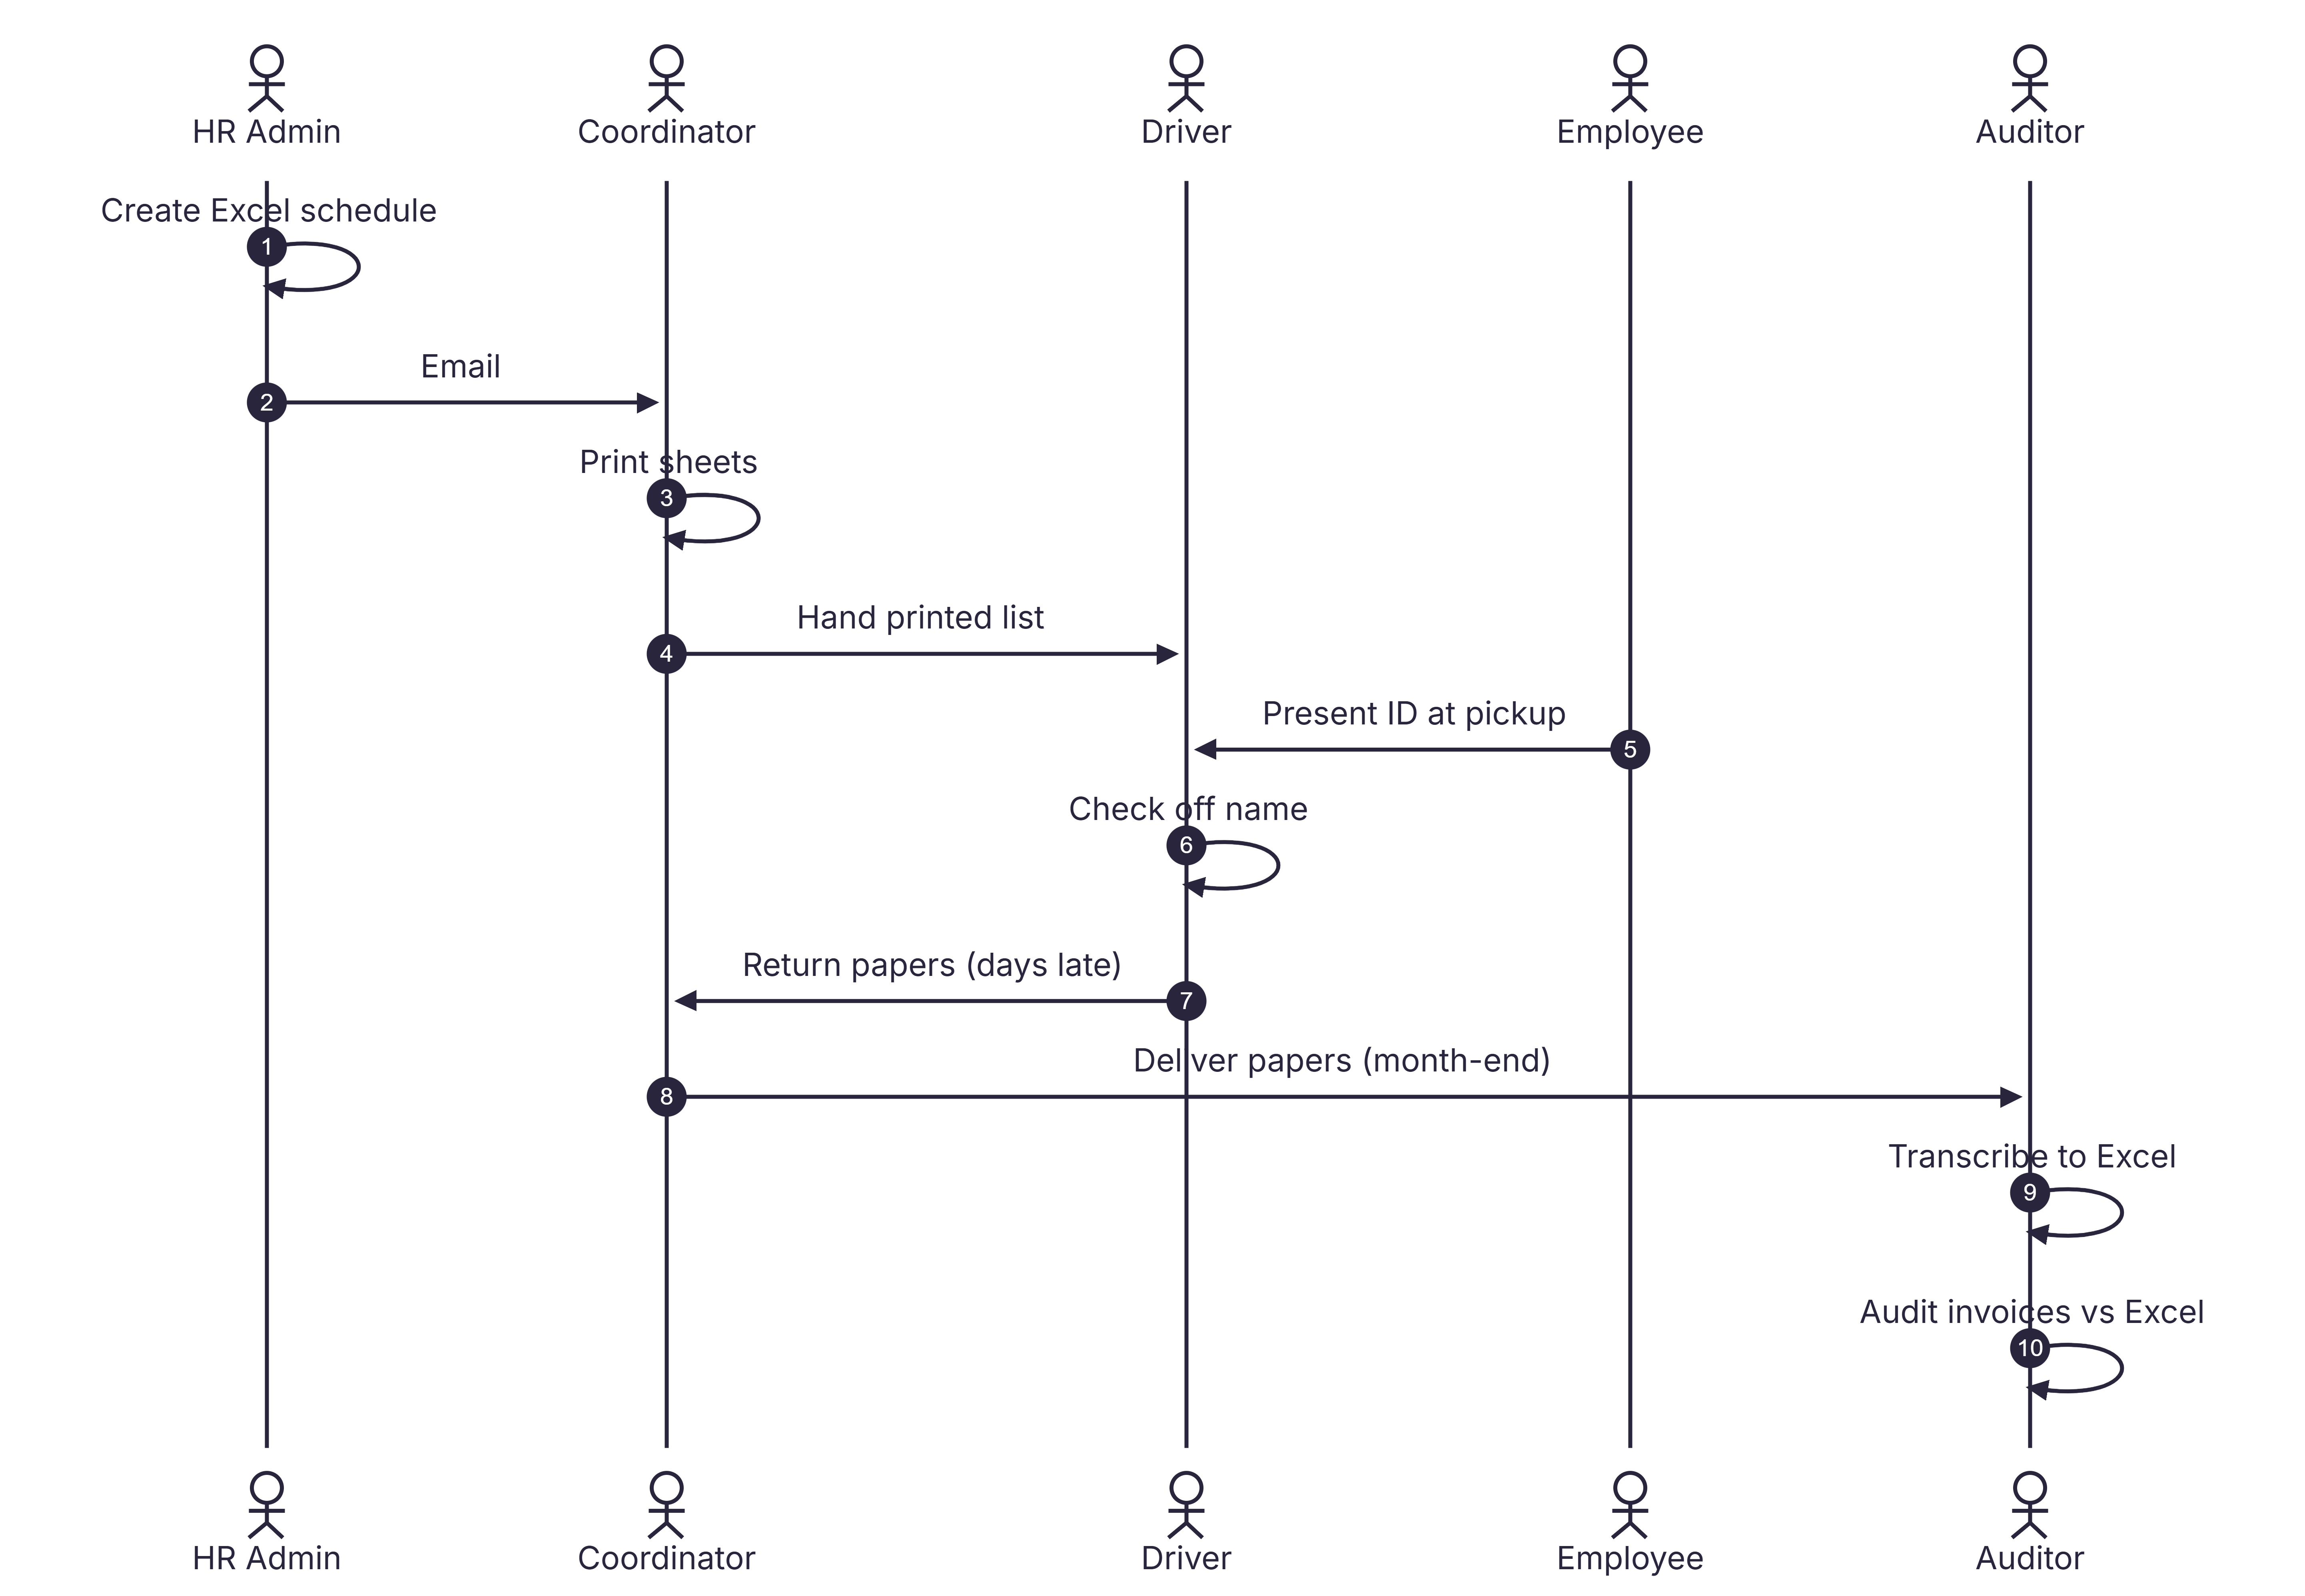
\includegraphics[width=1.2\textwidth,keepaspectratio]{figures/manual-boarding-sequence.png}}
  \caption{Manual Boarding and Attendance Process Sequence}
  \label{fig:manual_process_sequence}
\end{figure}

\subsection{Legacy Deployment Architecture}

In the legacy system, the technological architecture was restricted to a centralized database server with local office desktop fat-client instances. Information about transit execution remained isolated in physical logbooks and driver notes, with data manually entered long after the events occurred. Figure~\ref{fig:legacy_architecture} illustrates the legacy desktop-to-database flow and the lack of real-time network integration with the active fleet.

\begin{figure}[H]
  \centering
  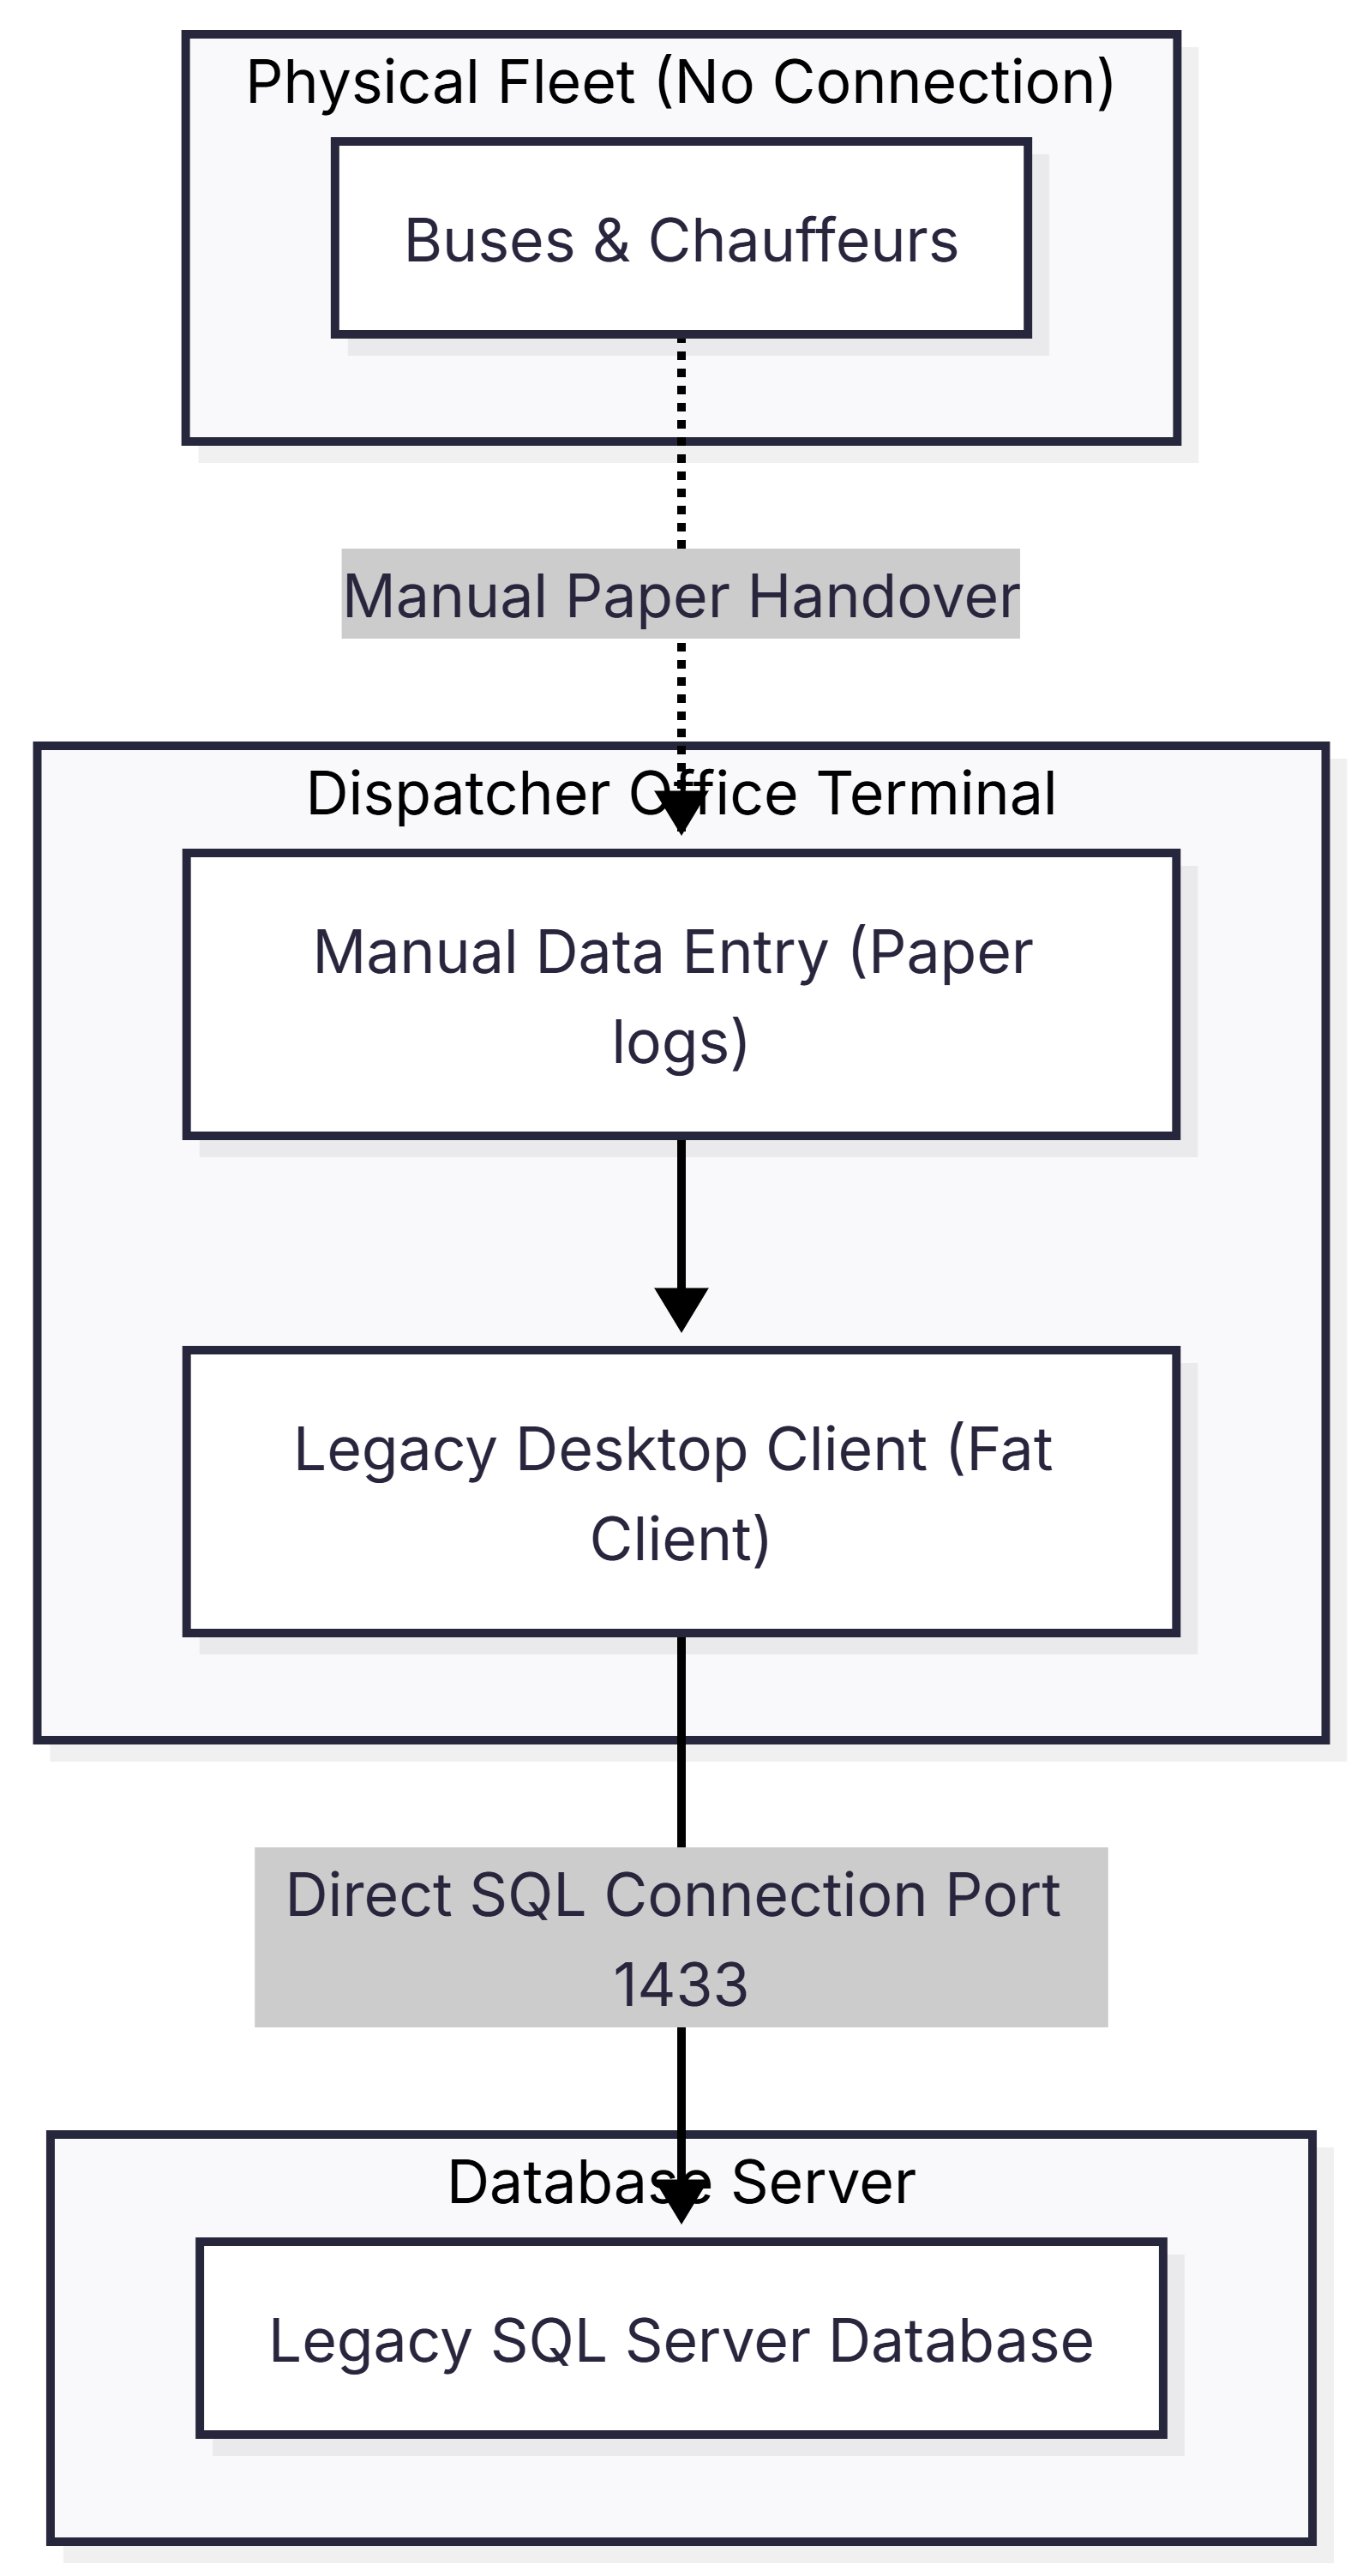
\includegraphics[width=0.85\textwidth,height=0.7\textheight,keepaspectratio]{figures/legacy-deployment-architecture.png}
  \caption{Legacy Deployment Architecture and Data Flow}
  \label{fig:legacy_architecture}
\end{figure}

\begin{table}[H]
  \small
  \centering
  \begin{tabularx}{\textwidth}{lXXXX}
    \toprule
    \textbf{Criteria} & \textbf{Manual Logbook} & \textbf{GPS Tracking} & \textbf{Office Biometrics} & \textbf{CST LePoint} \\
    \midrule
    HR Database Link & None & None & Direct (Gate only) & Fully Integrated \\
    Live Geolocation & None & Yes & None & Yes + Geofencing \\
    Boarding Audit & Paper sheets & None & None & Biometric/RFID check \\
    Route Audit & Visual inspect & Basic traces & None & Automatic geofencing \\
    Delay Predictions & None & None & None & ML ETA (FastAPI) \\
    Security \& RBAC & None & Weak & Strong & Granular RBAC \\
    Operational Cost & High labor & Medium (License) & Low & Low (Automated) \\
    \bottomrule
  \end{tabularx}
  \caption{Comparative Matrix of Transport and Attendance Tracking Solutions}
  \label{tab:comparative_matrix}
\end{table}

\section{Financial and Operational Impact of Transport Delays}

To understand the necessity of an integrated system, we must evaluate the financial and operational consequences of transit failures in industrial manufacturing environments:

\subsection{The Assembly Line Vacancy Problem}
In automotive parts assembly or electronic manufacturing plants operating on lean manufacturing models, production lines require a strict complement of operators to run safely. If a bus carrying 40 operators is delayed by 30 minutes, the assembly line cannot run at full speed. This leads to immediate bottlenecks, idle workstations downstream, and delayed product shipments.

\subsection{Concrete Delay Calculation}
Consider a standard Tunisian automotive wiring-harness factory with an hourly production value of $15,000$ TND. 
\begin{itemize}
  \item A bus breakdown occurs, delaying 40 specialized operators for $1.5$ hours.
  \item Because the operators are missing, a primary production line is halted.
  \item The financial cost of this halt is calculated as:
  \[\text{Loss} = \text{Hourly Production Value} \times \text{Duration} + \text{Overtime Compensations} = 15,000 \times 1.5 + 2,500 = 25,000 \text{ TND}\]
  \item In a manual environment, the plant manager is notified only after the shift starts, leaving no time to reassign workers from other lines.
\end{itemize}

By contrast, an automated real-time tracking system identifies when a vehicle stops moving on a scheduled route, evaluates the geofence breach, calculates the delayed ETA, and alerts dispatchers within 5 minutes, allowing managers to adjust shift patterns proactively.

\section{Detailed Operational Scenario}

Consider a morning shift breakdown scenario:
At 6:15 AM, a corporate bus carrying 40 factory operators scheduled for the 7:00 AM shift breaks down on a secondary highway.
\begin{itemize}
  \item \textbf{Roster State}: No live GPS track is active. The driver tries to call the dispatcher, but the line is busy.
  \item \textbf{Search and Rescue}: When the driver finally connects at 6:40 AM, they cannot provide exact coordinates. The dispatcher must call other vehicles to locate the broken bus.
  \item \textbf{Result}: The replacement bus reaches the site at 7:20 AM and delivers the workers to the factory at 7:50 AM, causing a major assembly line shutdown.
\end{itemize}

The sequence of events and communication breakdowns during this scenario is illustrated in Figure~\ref{fig:breakdown_scenario_timeline}.

\begin{figure}[H]
  \centering
  \begin{mermaid}[width=1.0\textwidth]
%%{init: { "theme": "redux", "themeVariables": { "fontSize": "28px", "actorFontSize": "28px", "noteFontSize": "26px", "messageFontSize": "26px", "fontFamily": "Arial, sans-serif" }, "sequence": { "actorWidth": 140, "actorHeight": 52, "boxWidth": 140, "messageMargin": 35 } }}%%
sequenceDiagram
    autonumber
    actor Driver as Driver
    actor Coord as Dispatcher
    actor Line as Manager
    actor Backup as Backup Driver

    Note over Driver: 06:15 AM: Bus breakdown
    Driver->>Coord: Call (No signal/Busy)
    Note over Driver, Coord: Delay: 25 mins
    Driver->>Coord: Report breakdown (06:40)
    Coord->>Driver: Ask coordinates
    Driver->>Coord: Verbal landmarks (imprecise)
    Coord->>Backup: Dispatch backup bus
    Note over Backup: Search delay: Locate bus
    Backup->>Driver: Reach breakdown (07:20)
    Note over Backup: Board employees
    Backup->>Line: Deliver workers (07:50)
    Line->>Line: Assembly line halted
    Note over Line: Loss: 25,000 TND
  \end{mermaid}
  \caption{Communication and Logistical Timeline during a Vehicle Breakdown}
  \label{fig:breakdown_scenario_timeline}
\end{figure}

\section{Limitations and Their Impact}

The critique of the manual and fragmented approach highlights several structural, operational, and technical limitations. These constraints directly degrade the logistical efficiency of industrial transit operations, causing significant financial waste, security vulnerabilities, and excessive administrative overhead.

\subsection{Detailed Technical and Operational Limitations}

The legacy system suffered from four fundamental operational and technical limitations:

\begin{itemize}
  \item \textbf{Desktop-Only Constraints}: The legacy application was deployed as a desktop fat-client directly wired to the SQL Server database. This localized setup meant that transit scheduling was only accessible from office workstations. Field dispatchers could not update schedules or driver details dynamically from the yard, managers had no remote operational visibility, and employees had no way to check bus schedules or routes.
  \item \textbf{Manual Paper Rosters}: Attendance check-ins relied entirely on printed sheets that drivers manually filled during boarding. This method is highly vulnerable to environmental damage (such as water or tearing), illegible handwriting, and data discrepancies. Furthermore, the attendance records remained in the vehicle for days or weeks before being manually transcribed, creating a massive latency in HR record updates.
  \item \textbf{Lack of Real-Time Geolocation}: With no real-time telemetry, the dispatcher office was completely blind to vehicle positions. The system served as a static database of planned circuits and driver contacts. If a bus was delayed, coordinators could only estimate its location and status by making direct phone calls to the driver, which is both dangerous while driving and prone to subjective reports.
  \item \textbf{Absence of Route Compliance Auditing}: There was no telemetry feedback loop to verify if drivers followed the scheduled circuits. Drivers could skip pickup points, take unauthorized detours, or deviate from planned paths to avoid traffic without the system registering any anomaly. This lack of auditing made it impossible to enforce route compliance or optimize transit loops.
\end{itemize}

\subsection{Business and Financial Impact on Logistics}

These technical limitations translate directly into measurable business and financial losses for the company:

\begin{itemize}
  \item \textbf{Delayed Shifts and Assembly Line Vacancy}: Tunisian manufacturing plants, such as automotive wiring-harness factories, operate on strict lean production models where workstations are tightly sequenced. A delay of a single bus carrying 30 or 40 technicians results in vacant assembly stations, slowing or halting the entire downstream line. The financial cost of such delays is severe, as calculated in the breakdown scenario ($25,000$ TND in idle labor and overtime recovery costs for a 1.5-hour delay).
  \item \textbf{Fuel Wastage and Unmonitored Mileage}: In the absence of automated route auditing, external transport contractors frequently bill for routes that are longer than necessary or routes they did not fully complete. Excessive engine idling, detours for driver personal errands, and unoptimized paths cause substantial fuel wastage and inflated subcontractor billing.
  \item \textbf{Security and Liability Risks}: Manual rosters do not offer secure verification of passengers. If a traffic accident or roadside emergency occurs, the company cannot quickly determine which employees were aboard the vehicle, creating serious regulatory and safety compliance liabilities. Furthermore, paper rosters are insecure and can easily be accessed by unauthorized personnel, exposing sensitive employee schedules and locations.
  \item \textbf{Administrative Burden and Invoice Auditing Delay}: At the end of every monthly billing cycle, administrative teams must manually type thousands of paper check-in entries into Excel files and cross-reference them with subcontractor invoices. This manual verification takes dozens of hours, is highly prone to human mathematical errors, and delays payments to transit providers.
\end{itemize}

\section{Identified Rooms for Improvement and Transition}

To resolve these operational difficulties and secure its logistics chain, Canadian System Technology requires a modernized, unified platform. The transition from the legacy desktop client to a cloud-ready web and mobile framework must focus on three core areas of improvement:

\begin{enumerate}
  \item \textbf{Real-Time Telemetry and Cartographic Supervision}: Replace static database registries with an active, web-based map interface. Using IoT modems installed in the buses, the system must process real-time coordinates via standard protocols (such as MQTT or HTTP) and dynamically plot vehicle positions, allowing dispatchers to monitor route progress and catch delays instantly.
  \item \textbf{Automated Attendance Tracking}: Replace manual paper sheets with digital boarding checks using RFID card scanners linked directly to the on-board IoT modems. As employees tap their company cards, the system must instantly validate their credentials, log their boarding status, and update the centralized HR database in real time.
  \item \textbf{Predictive Analytics and Intelligence}: Incorporate a machine learning layer to move from reactive scheduling to proactive management. The system should automatically query historical transit data and traffic conditions to calculate accurate Estimated Times of Arrival (ETA) for commuters, and analyze attendance traces to predict absenteeism risks before shifts begin.
\end{enumerate}

\section{Conclusion}

This chapter detailed the existing system and the limitations of manual transportation tracking workflows. It demonstrated the operational and financial impact of delays on lean manufacturing lines and identified key areas for improvement, establishing that a web-based, real-time, and predictive system is necessary to replace the legacy fat-client.

To implement this modernized system, a comprehensive set of specifications must be defined. The next chapter establishes the functional and non-functional requirements specification for the proposed CST LePoint platform.
